\documentclass[a4paper]{article}

\usepackage[english]{babel}
\usepackage[utf8]{inputenc}
\usepackage[english]{babel}
\usepackage{amsmath}
\usepackage{amsfonts}
\usepackage{amssymb}
\usepackage{enumitem}
\usepackage{listings}
\usepackage{hyperref}
\usepackage{graphicx}
\usepackage{epigraph}
\usepackage{comment}
\usepackage{longtable}
\title {Simplified Virtual Machine\\ INFSEN02-1, INFSEN22-1}
\author{ }
\date { }

\lstset
{
	basicstyle = \ttfamily\small,
	breaklines = true,
	frame = single
}

\begin{document}
\maketitle

The goal of this assignment is to realise a virtual machine, called \textit{Simplified Virtual Machine} (SVM) for a fictional assembly language (\textit{Assembly SVM}). This documents describes the specifications of the SVM and its assembly language. You will be provided with a template for an F\# solution containing a pre-built parser for the assembly language. The parser does the syntax analysis on a program written in SVM Assembly and outputs a data structure representing the program itself, which is described below. Your task is to build the interpreter, which is the component of the virtual machine that executes each statement in the assembly language and alters the state of the memory of the virtual machine. Your implementation must follow the following constraints:

\begin{itemize}
	\item You cannot change in any way the Parser (and thus the language specifications) of Assembly SVM.
	\item You cannot change the semantics (how the statements work) of Assembly SVM.
	\item You cannot use ANY imperative construct/statement other than commands to print on the shell. This means, for instance, no mutable variables, no loops, no mutable data structures, etc.
	\item If you want to use any language other than F\# you must implement a parser for Assembly SVM on your own using the same specifications.
\end{itemize}

\section{Architecture of the SVM}
The SVM is made of a set of memory locations, which index is called address. The total amount of memory locations available in the SVM can be specified by the user. Each memory location can contain integer, floating point, or string values (for simplicity, as this is different from hardware architectures and standard virtual machines where you only save bytes). Furthermore, unlike normal virtual machines, the values used in the assembly language are typed, meaning that the type compatibility is checked when executing a statement, in the same fashion as in high-level programming languages where, for example, you cannot sum a \texttt{string} with an \texttt{integer}.

The virtual machine has also 4 registers \texttt{reg1}, \texttt{reg2}, \texttt{reg3}, and \texttt{reg4}, that are special memory location used by the instructions to save temporary results or to contain temporary data. The data types contained in the registers can be the same as the main memory. It has also a special register, called \textit{Program Counter}, which contains the index of the current instruction to be executed.

Unlike low-level architectures, the program you have to execute is not saved in the memory but it is kept separate (thus the memory contains only the data and not the instructions the SVM has to execute).

\section{Interface with the Parser}
The Parser is defined in the Project \texttt{SVMParser} in the template solution. Please do not alter in any way this project otherwise the template will not work properly. The data structures you have to use to interface with the parser are defined in the file \texttt{AST.fs}. Import the module \texttt{SVMAST} after adding a reference to the \texttt{SVMParser} in the project you use for your own implementation to use the data structures. The parser processes the source file you want to load and creates a \texttt{Program} data structures, which is a list containing \texttt{Instructions}. The \texttt{Instruction} type is a discriminate union containing the definition of all the possible statements in Assembly SVM. Each \texttt{Instruction} can accept one or more arguments. Each \texttt{Argument} can be a literal (value) of type integer, floating point, or string, a \texttt{Register}, or a memory address. Some operators will accept only a \texttt{Register} as left argument (see the instruction specification below). \texttt{Registers} are represented as a discriminated union where each case represents the register itself.

\section{Syntax of Assembly SVM}
A program in Assembly SVM consists of one or more lines, each one containing a \textbf{single statement} in Assembly SVM. Thus, different statements must be written in different lines of the program. You can comment part of your program with the same syntax of Java/C++/C\# languages, that is // for single line comments and /* */ for multi-line comments. Also empty lines and white spaces are simply ignored by the parser, like in traditional programming languages. The language has three main categories of instructions:

\begin{itemize}
	\item \textit{Memory manipulation}: this statement takes two argments, one being the memory location/register to which you want to copy the data, and one being the data, memory location, or register you want to copy from.
	\item \textit{Operators}: they might be unary (with one argument) or binary (with two arguments).
	\item \textit{Labels}: They are identifiers that can be use to reference specific points of the program. To define a labels simply use the symbol \texttt{\#} followed by a variable name, which can be any alphanumerical sequence of characters starting with a letter. They can also contain the symbol '\textunderscore'. For example \texttt{\#hello\textunderscore world} is a valid label name, while \texttt{\#090error} is not a valid label name.
	\item \textit{Jump statements}: they alter the program counter by setting it to the line where a specific label is defined, thus allowing to implement the equivalent of \texttt{if-then-else} and \texttt{loops} of imperative programming.
\end{itemize}

The argument of an instruction can have three different types:

\begin{itemize}
	\item \textit{Literals}: they are constant values like numbers (\texttt{10}, \texttt{1053.23}) or strings (\texttt{"Hello world!"}).
	\item \textit{Memory addresses}: they are defined as integer numbers enclosed by square brackets, like \texttt{[100]}, which means ``the memory location at index 100''.
	\item \textit{Registers}: they are simply denoted with the keywords \texttt{reg1}, \texttt{reg2}, \texttt{reg3}, and \texttt{reg4}.
	\item \textit{Register references}: they are used when a register contains an integer number representing the address of a memory location, rather than a value. It is written just by enclosing the register keyword with square brackets. For instance, \texttt{[reg1]} means ``the content of the memory address stored in \texttt{reg1}. Thus, if the register contains the value 1000, this will use the content of the memory location at 1000.
\end{itemize}

\section{Instruction Behaviours}
When the SVM execute a statement, it performs 3 steps:

\begin{itemize}
	\item Check if the operands are type-compatible (according to the definition below). If they are not, it throws a runtime error.
	\item If the operand test succeeds, then it executes the instruction behaviour (see the table below).
	\item After executing the instruction, it increases the program counter by 1 \textbf{only if the instruction behaviour does not change the program counter, namely for the jump instructions}.
\end{itemize}

Below you find the details of all the operators accepted by the SVM language. Note that an argument which is an address can be either a \textit{Memory address} or a \texttt{Register reference}, as described above.

\begin{longtable}{|p{1cm}|p{2cm}|p{2cm}|p{5cm}|}
	\hline
	\textbf{Name} & \textbf{Arg1} & \textbf{Arg2} & \textbf{Behaviour} \\
	\hline
	NOP & None & None & This statement does not do anything and it leaves the state of the SVM unchanged. \\
	\hline
	MOV & Address or Register & Register, Address, or Constant & Copy the content or value of Arg2 into Arg1. If the memory address is out of range then it throws a runtime exception. \\
	\hline
	AND & Register & Register, Address, or Constant & If both arguments are $>=$ 0 then it stores 1 into Arg1, otherwise -1. It accepts only integer numbers, otherwise it raises a runtime exception. \\
	\hline
	OR & Register & Register, Address, or Constant & If both arguments are $<$ 0 then it stores -1 into Arg1, otherwise 1. It accepts only integer numbers, otherwise it raises a runtime exception. \\
	\hline
	NOT & Register & None & If the argument is non-negative, it stores -1 in Arg1, otherwise it stores 0. It accepts only an integer number, otherwise it raises a runtime exception. \\
	\hline
	MOD & Register & Register, Address, or Constant & It computes the modulus operation (remainder of the integer division) with Arg1 and Arg2 and stores the result in Arg1. It accepts only numerical arguments (integer or float), otherwise it raises a runtime exception. \\
	\hline
	ADD & Register & Register, Address, or Constant & It computes the sum operation with Arg1 and Arg2 and stores the result in Arg1. It accepts only numerical arguments (integer or float), otherwise it raises a runtime exception. \\
	\hline
	SUB & Register & Register, Address, or Constant & It computes the difference operation with Arg1 and Arg2 and stores the result in Arg1. It accepts only numerical arguments (integer or float), otherwise it raises a runtime exception. \\
	\hline
	MUL & Register & Register, Address, or Constant & It computes the multiplication operation with Arg1 and Arg2 and stores the result in Arg1. It accepts only numerical arguments (integer or float), otherwise it raises a runtime exception. \\
	\hline
	DIV & Register & Register, Address, or Constant & It computes the division operation with Arg1 and Arg2 and stores the result in Arg1. Note that with integers you do the integer division and with floats the floating point division. It accepts only numerical arguments (integer or float), otherwise it raises a runtime exception. \\
	\hline
	CMP & Register & Register, Address, or Constant & It compares the two arguments, returning -1 if Arg1 $<$ Arg2, 0 if they are equal, 1 if Arg1 $>$ Arg2. The result is stored in Arg1. It accepts only numerical values otherwise it raises a runtime exception. \\
	\hline
	\# & Id & None & The operator defines a label with the name specified in Arg1. It is not allowed to define labels with the same name, so in this case a runtime error should be raised. \\
	\hline
	JMP & Id & None & Jump at the point of the program where the label with the name in Arg1 is defined. This instruction modifies the program counter to do so. \\
	\hline
	JC & Id & Register & Jump at the point of the program where the label with the name in Arg1 is defined, if Arg2 is $>=$ 0. This instruction modifies the program counter to do so. \\
	\hline
	JEQ & Id & Register & Jump at the point of the program where the label with the name in Arg1 is defined, if Arg2 is 0. This instruction modifies the program counter to do so. \\
	\hline
\end{longtable}

\noindent
A further note on JC and JEQ: you use these instructions in combination with the CMP instruction. First you run CMP to compare the values, and then you use its result in the JC or JEQ instruction.

\vspace{0.5cm}
\noindent
\textbf{Example:} Consider the program

\begin{lstlisting}
if (x > 0)
{
  x -= 1;
}
else
{
  x += 1
}
\end{lstlisting}

\noindent
this will be translated in Assembly SVM, assuming that the value of \texttt{x} is stored at the memory address 15, as:

\begin{lstlisting}
//move the content of address 15 in reg1
mov reg1 [15]
//move the constant 0 in reg2
mov reg2 0 
//compare reg1 with reg2
cmp reg1 reg2
//negate the result (we want to jump if x <= 0)
not reg1
jc else reg1
//move back x into reg1 (it has been overwritten)
mov reg1 [15]
// x -= 1
sub reg1 1
//skip the else block 
jmp endif
#else
// x += 1
add reg1 1
#endif
//update the variable
mov [15] reg1
\end{lstlisting}

\section{Assignment}
Your task is to build the interpreter for Assembly SVM. This means that the template will generate a data structure representing the program, as defined in the module \texttt{SVMAST}, and you will have to build a software that executes that code, according to the instruction set defined above. Your program should be able to accept as input the source file written in Assembly SVM and the size (number of addresses) of the memory of the SVM you want to run the program on. The interpreter should raise an exception (which must be captured appropriately) in case of incompatible arguments, as described in the instruction behaviour. The output of the program should be a \textit{dump} of the SVM, which contains a visualization of the memory, the registers, and the program counter. Organize the memory display as a table with the memory locations content with 10 items per row. An example of a memory dump is shown in Figure \ref{fig:dump}.

\begin{figure}
	\centering
	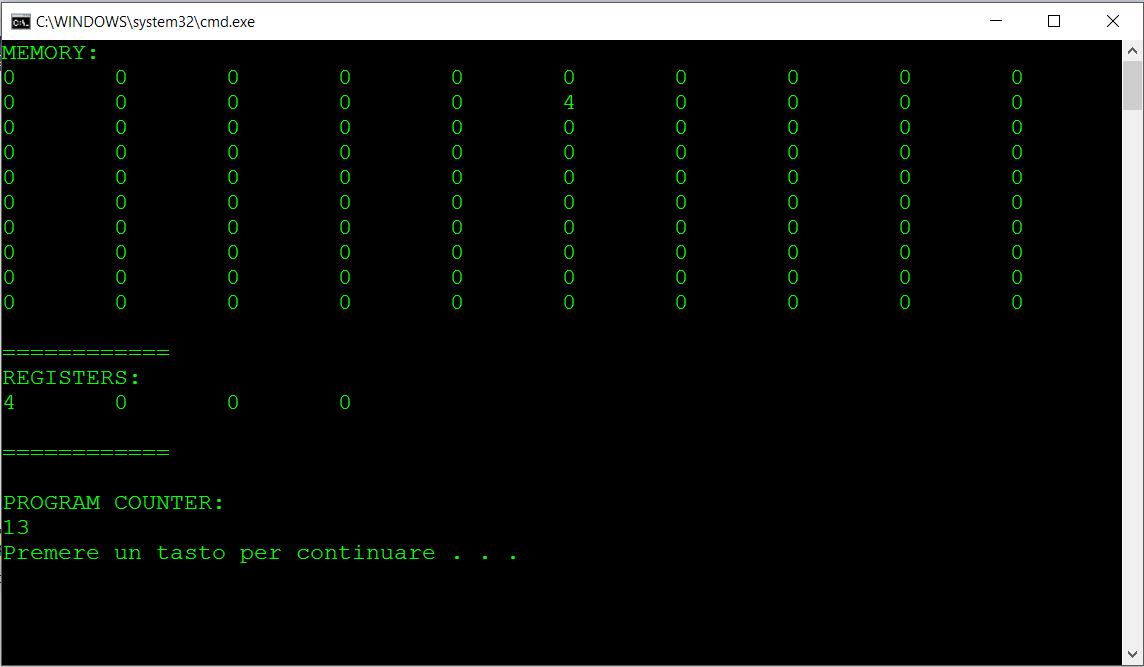
\includegraphics[width = \textwidth]{Figures/dump}
	\caption{Memory dump}
	\label{fig:dump}
\end{figure}

\noindent
Your implementation must observe the following rules:

\begin{itemize}
	\item You are not allowed to use any imperative constructs, other than statements that print on the standard output (such as \texttt{printfn}) and exceptions (\texttt{try-with} and \texttt{exception} definitions). This means no mutable values (\texttt{let mutable}), no variable assignments, such as \texttt{let mutable x = 0; x <- x + 1}, no \texttt{classes} (although immutable records are allowed), no \texttt{for} or \texttt{while} loops (you can use \textit{list comprehension} if you understand how they work, but this is out of the scope of the course), no arrays (only lists). You are allowed to use methods and properties in conjunction with  immutable records if they behave in an immutable way (so if they respect the constraints above).
	\item Your implementation should show that you know as much as possible the constructs of functional programming, so use as much as possible (of course where it makes senese) higher order functions, tuples, discriminated unions, immutable records, etc.
	\item Your solution must be tested with the examples included in the template but you are allowed to add your own programs written in Assembly SVM and present them.
	\item You are not allowed to change any part of the language definition, that is, the grammar, the syntactical representation generated by the Parser, and the instruction set.
\end{itemize}

\subsection{Evaluation}
Below you find how the evaluation matrix

\begin{longtable}{|c|c|p{8cm}|}
	\hline
	\textbf{Feature} & Maximum score & Details \\
	\hline
	SVM representation & 2 & The SVM is structured using a record with appropriate methods, properties, or functions implementing the functionalities (2 points). The SVM is implemented but without an explicit data type (1 point) or functions are not well structured according to the functional paradigm. 0 otherwise \\
	\hline
	Operators & 4 & Boolean, arithmetic, and comparison operators are implemented correctly (4 points). Operators are implemented but the exceptions are not handled properly or the argument by reference does not work (2 points). 0 otherwise. \\
	\hline
	Jump & 4 & Jump operators and labels are correctly implemented (4 points). Some jump operators are missing or not fully working (2 points). 0 otherwise. \\
	\hline  
\end{longtable}

\end{document}